% ======================================================================
% Master Manuscript — Part I (Reader's Guide) + Part II (Analytic Core) + Part III (Structural Corollaries)
% ======================================================================

\documentclass[11pt]{article}

% ------------------ Basic packages ------------------
\usepackage[a4paper,margin=1in]{geometry}
\usepackage{amsmath,amssymb,amsthm,mathtools}
\usepackage{microtype}
\usepackage{hyperref}
\usepackage{tabularx,booktabs,array}
\usepackage{enumitem}
\usepackage{needspace}
\usepackage{tikz}

% ------------------ Theorem styles ------------------
\newtheorem{theorem}{Theorem}[section]
\newtheorem{lemma}[theorem]{Lemma}
\newtheorem{corollary}[theorem]{Corollary}
\newtheorem{proposition}[theorem]{Proposition}
\theoremstyle{remark}
\newtheorem{remark}[theorem]{Remark}

% ------------------ Tabularx helper column ------------------
\newcolumntype{L}{>{\raggedright\arraybackslash}X}

% ------------------ Macros: frames, functions, projectors ------------------
\newcommand{\C}{\mathbb{C}}
\newcommand{\R}{\mathbb{R}}
\newcommand{\Z}{\mathbb{Z}}
\newcommand{\D}{\mathbb{D}}
\newcommand{\Real}{\operatorname{Re}}
\newcommand{\Imag}{\operatorname{Im}}
\newcommand{\zetaTwo}{\zeta_2}
\newcommand{\LambdaTwo}{\Lambda_2}
\newcommand{\LamTwo}{\LambdaTwo}
\newcommand{\Afac}{A_2}
\newcommand{\chiTwo}{\chi_2}
\newcommand{\Podd}{P_{\mathrm{odd}}}
\newcommand{\Peven}{P_{\mathrm{even}}}
\newcommand{\Ucore}{U}
\newcommand{\UR}{U_{\mathrm{R}}}
\newcommand{\UL}{U_{\mathrm{L}}}
\newcommand{\Ecomp}{E}
\newcommand{\Gout}{G_{\mathrm{out}}}
\newcommand{\Zloc}{Z_{\mathrm{loc}}}
\newcommand{\Arg}{\operatorname{Arg}}
\newcommand{\sgn}{\operatorname{sgn}}
\newcommand{\ii}{\mathrm{i}}

% ------------------ Optional overview block ------------------
\newenvironment{Overview}{\begin{quote}\itshape}{\end{quote}}

% ------------------ Title page ------------------
\title{\Large A Height--Local Width--2 Program for Excluding Off--Axis Quartets\\[2pt]
\large Analytic Tail \& Certified Outer/Rouch\'e Criterion}
\author{Dylan Anthony Dupont}
\date{\today}

\begin{document}
\maketitle

\begin{abstract}
\noindent
This paper is organized in three parts. 
\textbf{Part~I} (Reader’s Guide) reduces the Riemann Hypothesis (RH) to a height--local statement in the width--2 frame: \emph{RH $\Leftrightarrow$ $a(m)=0$ at each nontrivial height $m$}, while recording non--load--bearing structural scaffolding.
\textbf{Part~II} gives a self--contained, boundary--only analytic proof that the per--height tilt satisfies $a(m)=0$ at every nontrivial height using a disc--based $L^2$ upper envelope and an $L^2$ lower envelope via allocation $+$ restricted contour $+$ Jensen, and provides a rigorous Outer/Rouch\'e Certification Path with explicit domains and symbolic constants (``shape--only'' vs.\ residual).
\textbf{Part~III} promotes the toolbox identities to structural corollaries once $a(m)=0$ is established, with full constructions and proofs.
\end{abstract}

\setcounter{tocdepth}{2}
\tableofcontents

% ======================================================================
% Part I — Reader’s Guide / Motivation, Reduction & Implications
% ======================================================================
\section*{Part I --- Reader’s Guide / Motivation, Reduction \& Implications}
\addcontentsline{toc}{section}{Part I --- Reader’s Guide / Motivation, Reduction \& Implications}

\paragraph{What this section is (and is not).}
\emph{What it does.} It introduces modulated frames and the width--2 normalization, defines the centered $a$--lens that measures horizontal tilt at a fixed height, and reduces RH to the height--local target $a(m)=0$ for each nontrivial height $m$. It also records the structural toolbox (projectors, rectifier, canonical stream, recurrence, curvature extractor, seed$\to$rectifier) and explains how these become consequences once $a(m)=0$ is proved.

\noindent\emph{What it does not do.} It contains no analytic estimates and no proofs. The hinge unitarity fact and all bounds are proved later; this Guide is not used by the analytic part.

\subsection*{1) Modulated frames and the width--2 pivot}
For $f>0$ define the modulated family $\zeta_f(s):=\zeta(s/f)$ with completed form
\[
\Lambda_f(s)=\pi^{-\,s/(2f)}\,\Gamma\!\Big(\frac{s}{2f}\Big)\,\zeta_f(s),
\]
so $\Lambda_f$ is entire and satisfies $\Lambda_f(s)=\Lambda_f(f-s)$. Equivalently, $\zeta_f(s)=A_f(s)\,\zeta_f(f-s)$ with $A_f(s)A_f(f-s)\equiv1$.

\smallskip
\noindent\textbf{Width--2 normalization.} Put $u:=(2/f)\,s$. Then
\[
\zetaTwo(u):=\zeta(u/2),\qquad
\LambdaTwo(u):=\pi^{-u/4}\Gamma(u/4)\,\zeta(u/2),\qquad
\LambdaTwo(u)=\LambdaTwo(2-u).
\]
The non--completed FE reads $\zetaTwo(u)=\Afac(u)\,\zetaTwo(2-u)$.
In the open strip $0<\Real u<2$ and $\Imag u\neq0$, $\Afac$ is analytic and nonvanishing.

\smallskip
\noindent\textbf{Partner map.} On $\Imag u>0$, FE $+$ conjugation gives the involution $J(u)=2-\overline{u}$.

\smallskip
\noindent\textbf{Hinge unitarity (deferred).} The statement ``$|\chiTwo(u)|=|\Afac(u)|^{-1}=1$ iff $\Real u=1$'' is proved in Part~II (Hinge--Unitarity, Theorem~\ref{thm:hinge}); a complete proof is given in Appendix~\ref{app:hinge}.

\subsection*{2) Centered $a$--lens and the quartet}
Let $v:=u-1$ and $\Ecomp(v):=\LambdaTwo(1+v)$. Then $\Ecomp(v)=\Ecomp(-v)=\overline{\Ecomp(\overline v)}$.

\smallskip
\noindent\textbf{Nontrivial height.} A ``nontrivial height'' $m>0$ means: $m$ occurs as the imaginary part of a nontrivial zero $s=\tfrac12+\ii m/2$. The reduction shows that whenever such an $m$ occurs, the associated tilt must satisfy $a(m)=0$.

\smallskip
\noindent\textbf{Tilt at height $m$.} At fixed $m>0$, set
\[
\UR(m;a)=1+a+\ii m,\qquad \UL(m;a)=1-a+\ii m,\qquad a\in[0,1).
\]
In the centered frame, the dial points are $\pm(a+\ii m)$. The partner map $J$ swaps $\UR\leftrightarrow \UL$.

\smallskip
\noindent\textbf{Quartet.} Conjugation and FE reflection generate the quartet $\{\,1\pm a\pm \ii m\,\}$ at height $m$.

\subsection*{3) Why width--2: slope invariance}
If the columns collapse at height $m$ ($a=0$), the point is $u=1+\ii m$ and its slope is $\Imag u/\Real u = m/1=m$. Rescaling to any frame $s=(f/2)\,u$ preserves the slope:
\[
\frac{\Imag s}{\Real s}=\frac{(f/2)\,m}{f/2}=m.
\]

\subsection*{4) Height--local reduction of RH}
Fix $m>0$ and write $\UR=1+a+\ii m$, $\UL=1-a+\ii m$. The purely algebraic equivalences:
\begin{itemize}
  \item (PHU--1) Column equality: $\Real \UR=\Real \UL \iff a=0$.
  \item (PHU--2) Ray lock: $\Imag \UR/\Real \UR=\Imag \UL/\Real \UL\iff a=0$.
  \item (PHU--3) Hinge form: $\UR=\UL=1+\ii m$.
\end{itemize}
\emph{Reduction target.} RH $\iff$ for every nontrivial height $m>0$, $a(m)=0$. Part~II proves this per--height collapse.

\subsection*{5) Box alignment and hand--off}
Define
\[
B(\alpha,m,\delta)=[\alpha-\delta,\alpha+\delta]\times[m-\delta,m+\delta],\qquad
\delta:=\eta\,\alpha/(\log m)^2,\ \ \eta\in(0,1).
\]
When $\alpha=\pm a$, the dial points $\pm(a+\ii m)$ lie on the box’s horizontal centerline.

\subsection*{6) Parity gating (interpretive only)}
In width--2,
\[
\zetaTwo(u)=\Afac(u)\,\zetaTwo(2-u),\quad
\Afac(u)=2^{u/2}\,\pi^{\,u/2-1}\,\sin\!\Big(\frac{\pi u}{4}\Big)\,\Gamma\!\Big(1-\frac{u}{2}\Big).
\]
On $0<\Real u<2$, $\Afac(u)\neq0$; its sine zeros are real only. Thus \emph{inside the open strip only $\zetaTwo$ can vanish}. A lattice split via
\[
\Podd(n)=\tfrac{1-\cos(\pi n)}{2},\quad
\Peven(n)=\tfrac{1+\cos(\pi n)}{2}
\]
models the odd (nontrivial) vs even (trivial ladder) dichotomy.

\subsection*{7) Toolbox $\to$ structural consequences (\emph{see Part~III})}
The items below are not inputs to the analytic proof. After Part~II proves $a(m)=0$ for all $m>0$, they become \emph{Structural Corollaries} recorded and proved in Part~III: canonical columns, collapsed canonical stream (parity and trigonometric faces), single--frequency collapse, self--indexed recurrence, and curvature extractor.

% ======================================================================
% Part II — Analytic Core (self-contained; boundary-only)
% ======================================================================
\section*{Part II --- Self-Contained Boundary--Only Contradiction on Aligned Boxes}
\addcontentsline{toc}{section}{Part II --- Self-Contained Boundary--Only Contradiction on Aligned Boxes}

In the width-2 frame $u=2s$, $v=u-1$, let $\LamTwo(u)=\pi^{-u/4}\Gamma(u/4)\zeta(u/2)$ and $E(v)=\LamTwo(1+v)$. We exclude off-axis quartets $\{\pm a\pm \ii m\}$ by:
\begin{enumerate}[label=(\arabic*)]
\item an analytic tail (uniform in $\alpha$): short-side forcing $\ge \pi/2$; residual bound for $F=E/\Zloc$ with perimeter $8\delta$; disc-based $L^2$ boundary-to-midpoint estimate with shape-only constants;
\item a rigorous Outer/Rouch\'e Certification Path: interval arithmetic on $\partial B$ + validated Poisson + Lipschitz grid$\to$continuum enclosure $\Rightarrow \sup_{\partial B}\!\big|E-\Gout\big|/|\Gout|<1$ $\Rightarrow$ zero-free box, then inner collapse and stitching.
\end{enumerate}

% ---- Box schematic (one-page map) ----
\begin{figure}[htbp]\centering
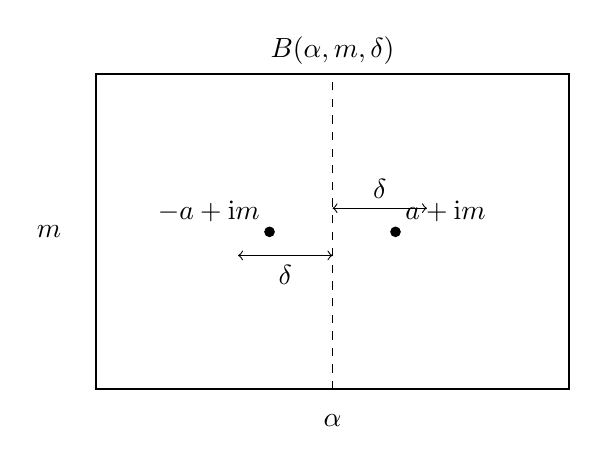
\begin{tikzpicture}[scale=1.0]
  \draw[thick] (0,0) rectangle (6,4);
  \draw[dashed] (3,0) -- (3,4);
  \node at (3,-0.4) {$\alpha$};
  \node at (-0.6,2) {$m$};
  \draw[fill] (3.8,2) circle (0.06) node[above right] {$a+\mathrm{i}m$};
  \draw[fill] (2.2,2) circle (0.06) node[above left] {$-a+\mathrm{i}m$};
  \draw[<->] (3,2.3) -- (4.2,2.3) node[midway,above] {$\delta$};
  \draw[<->] (3,1.7) -- (1.8,1.7) node[midway,below] {$\delta$};
  \node at (3,4.3) {$B(\alpha,m,\delta)$};
\end{tikzpicture}
\caption*{Aligned box $B(\alpha,m,\delta)$ with dials $\pm(a+\mathrm{i}m)$ on the centerline and short vertical sides at $\alpha\pm\delta$.}
\end{figure}

% ---------------------------------------------------
\Needspace{30\baselineskip}
\section*{Symbols \& Provenance (at a glance)}
% ---------------------------------------------------

\renewcommand{\arraystretch}{1.12}
\noindent\textit{Notation hygiene.} Reserve $\psi$ for the digamma function and write $\varphi:\D\to B$ for conformal maps.

\medskip
\begin{tabularx}{\textwidth}{@{}p{4.2cm} L L@{}}
\toprule
\textbf{Symbol} & \textbf{Definition / role} & \textbf{Provenance / why this form}\\
\midrule
$u=2s$, $v=u-1$ & Width-2 frame centered at $\Real u=1$ & Centers functional equation symmetry\\\midrule
$\LamTwo(u)=\pi^{-u/4}\Gamma\!\big(\frac{u}{4}\big)\zeta\!\big(\frac{u}{2}\big)$ & Completed object & Standard; FE for $\LamTwo$; width-2 transport\\\midrule
$E(v)=\LamTwo(1+v)$ & Workhorse in $v$-plane & Even \& conjugate-symmetric: $E(v)=E(-v)=\overline{E(\bar v)}$\\\midrule
$\zeta_2(u)=\zeta(u/2)$ & Width-2 zeta & Used in FE and hinge law\\\midrule
$\chiTwo(u)$ & FE factor inverse & $\chiTwo(u)=\pi^{u/2-1/2}\,\Gamma((2-u)/4)/\Gamma(u/4)$\\\midrule
$B(\alpha,m,\delta)$ & $[\alpha-\delta,\alpha+\delta]\times[m-\delta,m+\delta]$ & Square (width \& height $2\delta$) centered at $(\alpha,m)$\\\midrule
$\alpha\in(0,1]$ & Horizontal center & Left dial handled by reflection $w=-v$\\\midrule
$m\ge 10$ & Height parameter & Ensures uniform DLMF/Titchmarsh/Ivi\'c regimes\\\midrule
$\delta=\dfrac{\eta\,\alpha}{(\log m)^2}$, $\eta\in(0,1)$ & Half-side length of $B$ & Balances forcing vs residual $O(\delta\log m)$\\\midrule
$\partial B$, $I_\pm$, $Q$ & Boundary / short verticals / quiet horizontals & For forcing budgets and $L^2$ control\\\midrule
$\Zloc(v)=\prod_{|\Imag\rho-m|\le 1}(v-\rho)^{m_\rho}$ & Local zero/pole factors & De-singularizes $E$ near $\partial B$\\\midrule
$F=E/\Zloc$ & Residual analytic factor & Lemma~\ref{lem:residual} (constants symbolic)\\\midrule
$G(v)=\dfrac{E(1+v)}{E(1-v)}$ & Odd-lane quotient & Links to hinge via two-point identity\\\midrule
$\Gout=e^{U+\ii V}$ & Outer with $|\,\Gout\,|=|E|$ on $\partial B$ & $U=\log|E|\in C(\overline B)$ solves Dirichlet; $V$ harmonic conjugate\\\midrule
$W=E/\Gout$ & Inner quotient ($|W|=1$ a.e. on $\partial B$) & Collapses to unimodular constant upon certification\\\midrule
$v_\pm^\star=\pm(a+\ii m)$ & Dial pair on centerline & Points of evaluation in the tail\\\midrule
$Z_{\rm pair}(v)$ & $(v-(a+\ii m))(v-(-a+\ii m))$ & Short-side forcing on $I_+$\\\midrule
$\Gamma_\lambda$ & Central $\lambda\delta$ sub-arcs + tiny joins & Restricted contour (zero forcing)\\\midrule
$B_{\rm core}(a,m;\lambda)$ & Dial-centred core box & Zero location forced by $\Gamma_\lambda$\\\midrule
$K_{\rm alloc}^{(\star)}(\lambda)$ & Allocation coefficient & Shape-only; Lemma~\ref{lem:allocL2}\\\midrule
$c_0=\frac{1}{4\pi}\log(2\sqrt{2})$ & Dial deficit constant ($\lambda=\tfrac12$) & From Jensen at dial; Lemma~\ref{lem:jensen-dial}\\\midrule
$C_{\mathrm{up}}$ & Upper-envelope constant & Shape-only; Lemma~\ref{lem:upper-disc}\\\midrule
$C_h''$ & Horizontal budget constant & Shape-only; Lemma~\ref{lem:corezero}\\
\bottomrule
\end{tabularx}

\medskip
\noindent\textit{Sources.} Digamma: DLMF §5.5, §5.11. $\zeta'/\zeta$: Titchmarsh §14; Ivi\'c Ch.~9. Lipschitz Hilbert/Cauchy and boundary traces: Coifman--McIntosh--Meyer (1982); Duren; Garnett.

% ---------------------------------------------------
\section{Frames, symmetry, and the hinge law}\label{sec:frames}
% ---------------------------------------------------

We work in $u=2s$, $v=u-1$, with
\[
\LamTwo(u)=\pi^{-u/4}\Gamma\!\Big(\frac{u}{4}\Big)\zeta\!\Big(\frac{u}{2}\Big),
\qquad
E(v):=\LamTwo(1+v).
\]
Then $E(v)=E(-v)=\overline{E(\bar v)}$; off-axis zeros appear as quartets $\{\pm a\pm \ii m\}$.

\begin{theorem}[Hinge--Unitarity]\label{thm:hinge}
Let $\zeta_2(u)=\zeta(u/2)$ and $\zeta_2(u)=A_2(u)\,\zeta_2(2-u)$ with
\[
\chiTwo(u):=A_2(u)^{-1}=\pi^{u/2-1/2}\frac{\Gamma\big(\frac{2-u}{4}\big)}{\Gamma\big(\frac{u}{4}\big)}.
\]
For fixed $t\neq 0$, define $f(\sigma)=\log|\chi_2(\sigma+\ii t)|$. Then
\[
f'(\sigma)=\tfrac12\log\pi-\tfrac12\,\Real\psi\!\Big(\tfrac{\sigma+\ii t}{4}\Big)
-\tfrac14\,\Real\!\Big[\pi\cot\!\Big(\tfrac{\pi}{4}(\sigma+\ii t)\Big)\Big].
\]
Moreover,
\[
\big|\Real\!\big[\pi\cot(x+\ii y)\big]\big|\;\le\;\frac{\pi}{\cosh(2y)-1}.
\]
Taking $x=\frac{\pi}{4}\sigma$, $y=\frac{\pi}{4}|t|$, for $|t|\ge m_1/2$ (Appendix~\ref{app:firstheight-certified}) the cotangent term is $<10^{-8}$. Using vertical-strip bounds,
\[
\Real\psi\!\Big(\frac{\sigma+\ii t}{4}\Big)\ \ge\ \log\!\Big(\frac{|t|}{4}\Big)-\frac{2}{|t|},
\]
hence $f'(\sigma)<0$ on $\R$ for all such $t$. Since $f(1)=0$, $|\chi_2(u)|=1$ iff $\Real u=1$. For $|t|<m_1/2$ the range is covered by the certified base band (Appendix~\ref{app:firstheight-certified}). A complete proof is provided in Appendix~\ref{app:hinge}.
\end{theorem}

% ---------------------------------------------------
\section{Boxes, de-singularization, residual control, and forcing}\label{sec:boxes}
% ---------------------------------------------------

Fix $m\ge 10$, $\alpha\in(0,1]$, and
\begin{equation}\label{eq:box-delta}
B(\alpha,m,\delta)=\big[\alpha-\delta,\alpha+\delta\big]\times\big[m-\delta,m+\delta\big],
\qquad
\delta=\frac{\eta\,\alpha}{(\log m)^2},\ \ \eta\in(0,1).
\end{equation}

\paragraph{Short boxes stay in $\Real v>0$.}
Since $\eta/(\log m)^2<1$, one has $\delta<\alpha$; thus the left edge $\alpha-\delta>0$ and $B\subset\{\Real v>0\}$.

\paragraph{De-singularization on $\partial B$.}
Let
\begin{equation}\label{eq:Zloc}
\Zloc(v)=\prod_{\rho:\,|\Imag\rho-m|\le 1}(v-\rho)^{m_\rho},\qquad
F(v):=\frac{E(v)}{\Zloc(v)}.
\end{equation}
Then $F$ is analytic and zero-free on a neighborhood of $\partial B$.

\paragraph{Boundary contact convention.}
If a zero/pole meets $\partial B$, shrink $\delta$ by $1-\varepsilon$ or shift $\alpha$ by $O(\delta)$; all constants remain stable.

\begin{lemma}[Residual envelope]\label{lem:residual}
On $\partial B$,
\begin{equation}\label{eq:residual-sup}
\sup_{\partial B}\Big|\frac{F'}{F}\Big|\ \le\ C_1\log m + C_2,
\end{equation}
and
\begin{equation}\label{eq:residual-perimeter}
\big|\Delta_{\partial B}\arg F\big|\ \le\ 8\delta\,\big(C_1\log m+C_2\big).
\end{equation}
\begin{proof}
On $1/2\le\sigma\le 1$ and $t\ge 3$, Titchmarsh (rev.\ Heath--Brown) and Ivi\'c give
\(
\frac{\zeta'}{\zeta}(\sigma+\ii t)=\sum_{|\Imag\rho-t|\le 1}\frac{1}{\sigma+\ii t-\rho}+O(\log t)
\).
Transport $s=(\sigma+\ii t)$ to width--2 ($u=2s$), and write $v=u-1$. Removing the local factors with $Z_{\rm loc}$ deletes the principal parts on $|\Imag\rho-m|\le 1$, so on a neighborhood of $\partial B$ the residual $F=E/Z_{\rm loc}$ has
\(
\frac{F'}{F}=O(\log m)
\),
with absolute constants $C_1,C_2>0$. The perimeter bound follows from
\(
\Delta_{\partial B}\arg F=\int_{\partial B}\partial_\tau\arg F\,ds
\)
and \(
|\partial B|=8\delta
\).
\end{proof}
\end{lemma}

\begin{lemma}[Logarithmic derivatives on $\partial B$]\label{lem:bridge-logs}
On $\partial B$,
\[
\frac{E'}{E}=\frac{F'}{F}+\frac{(Z_{\rm loc})'}{Z_{\rm loc}},\qquad
\sup_{\partial B}\Big|\frac{E'}{E}\Big|
\ \le\ \sup_{\partial B}\Big|\frac{F'}{F}\Big|+\sum_{\rho:\,|\Imag\rho-m|\le 1}\ \sup_{v\in\partial B}\frac{m_\rho}{|v-\rho|}\,.
\]
\begin{proof}
Differentiate $E=F\,Z_{\rm loc}$ and take suprema termwise; finiteness is guaranteed by the boundary-contact convention.
\end{proof}
\end{lemma}

\begin{lemma}[Short-side forcing]\label{lem:short-side}
Let $Z_{\rm pair}(v)=(v-(a+\ii m))(v-(-a+\ii m))$. On
\[
I_+=\{\alpha+\ii y:\ |y-m|\le \delta\},\quad\text{with }|\alpha-a|\le\delta,
\]
one has
\begin{equation}\label{eq:short-side}
\Delta_{I_+}\arg Z_{\rm pair}
=2\arctan\frac{\delta}{|\alpha-a|}+2\arctan\frac{\delta}{\alpha+a}\ \ge\ \frac{\pi}{2}.
\end{equation}
\begin{proof}
The increment of $\arg(v-(\pm a+\ii m))$ as $y$ runs from $m-\delta$ to $m+\delta$ is
$2\arctan(\delta/|\alpha\mp a|)$; the sum yields the display. If $|\alpha-a|\le\delta$, the first addend is at least $\pi/2$; the second is nonnegative since $\alpha+a>0$.
\end{proof}
\end{lemma}

% ---------------------------------------------------
\section{Boundary-only criteria, bridges, and corner interpolation}\label{sec:criteria}
% ---------------------------------------------------

\subsection{Two-point Schur/outer criterion}\label{subsec:schur-criterion}

Let $\varphi:\D\to B$ be conformal with $\varphi(0)$ the box center and avoiding corners at two marked points. Define
\begin{equation}\label{eq:schur-def}
G(v):=\frac{E(1+v)}{E(1-v)},\qquad \Phi:=(G/H)\circ\varphi,
\end{equation}
where $H$ is an \emph{outer majorant}: choose $M\in C(\partial B)$ with $M\ge |G|$ a.e., let $U$ solve Dirichlet with data $\log M$, fix a harmonic conjugate $V$, and set $H=e^{U+\ii V}$.

\begin{proposition}[Two-point Schur pinning]\label{prop:schur-pin}
If $\Phi\in H^\infty(\D)$ with $\|\Phi\|_\infty\le 1$, and two non-corner boundary points $\zeta_\pm$ have a.e.\ unimodular limits while an arc $A\subset\partial\D$ has $\operatorname*{ess\,sup}_{A}|\Phi|\le 1-\varepsilon$, then for any $z\in\D$ with $\omega_z(A)\ge\omega_*>0$,
\[
|\Phi(z)|\ \le\ 1-\kappa,\quad \kappa=\kappa(\varepsilon,\omega_*)>0,
\]
hence $|G(\varphi(z))|\le (1-\kappa)|H(\varphi(z))|$.
\begin{proof}
By outer majorant construction, $|\Phi|=|G|/|H|\le 1$ a.e.\ on $\partial\D$. On the arc $A$ the boundary modulus is $\le 1-\varepsilon$. By the Poisson representation and the maximum modulus principle for $H^\infty(\D)$, interior values satisfy $|\Phi(z)|\le (1-\varepsilon)^{\omega_z(A)}\le 1-\kappa$ for $\kappa:=1-(1-\varepsilon)^{\omega_*}$. Transport via $\varphi$ gives the bound on $|G|$.
\end{proof}
\end{proposition}

\begin{lemma}[Two-point link for $|G|$ and $|\chi_2|$]\label{lem:G-chi-link}
For $v=a+\ii m$,
\begin{equation}\label{eq:G-chi-link}
|G(v)|=\big|\chi_2(1+v)\big|\cdot R(v),\qquad R(-v)=R(v)^{-1},
\end{equation}
hence
\begin{equation}\label{eq:G-chi-product}
|G(a+\ii m)|\,|G(-a+\ii m)|
=\big|\chi_2(1+a+\ii m)\big|\,\big|\chi_2(1-a+\ii m)\big|.
\end{equation}
\begin{proof}
Expand $E(1\pm v)$ from $\LamTwo$; collect $\pi$ and $\Gamma$ factors to form $\chi_2$ and a residual $R$. Multiplying at $\pm v$ cancels $R$, giving \eqref{eq:G-chi-product}.
\end{proof}
\end{lemma}

\subsection{Outer/Rouch\'e Certification Path}\label{subsec:rouche-criterion}

Let $U$ solve Dirichlet on $B$ with boundary data $\log|E|$, $V$ harmonic conjugate, and
\[
\Gout:=e^{U+\ii V}.
\]
\begin{proposition}[Outer/Rouch\'e criterion]\label{prop:rouche-criterion}
If
\begin{equation}\label{eq:rouche-ratio}
\sup_{v\in\partial B}\frac{|E(v)-\Gout(v)|}{|\Gout(v)|}\ <\ 1,
\end{equation}
then $E$ is zero-free in $B$. Consequently $W:=E/\Gout$ is analytic and nonvanishing with $|W|=1$ a.e.\ on $\partial B$.
\begin{proof}
Rouch\'e's theorem on simply connected domains applies since $\Gout$ is nonvanishing; the modulus equality $|\Gout|=|E|$ a.e.\ along $\partial B$ follows by construction. Hence $E$ and $\Gout$ have identical zero counts. As $\Gout$ has none, neither does $E$.
\end{proof}
\end{proposition}

\begin{proposition}[Bridge~1: inner collapse]\label{prop:bridge1}
Under \eqref{eq:rouche-ratio}, $\log|W|$ is harmonic with vanishing boundary trace, hence $|W|\equiv 1$ and $W\equiv e^{\ii\theta_B}$ by the open mapping theorem.
\end{proposition}

\begin{proposition}[Bridge~2: stitching]\label{prop:bridge2}
If $B_1,B_2$ overlap and $W\equiv e^{\ii\theta_{B_j}}$ on $B_j$, then $e^{\ii\theta_{B_1}}=e^{\ii\theta_{B_2}}$ on the overlap; a tiled band inherits a single unimodular phase.
\end{proposition}

\subsection{Corner outer interpolation}\label{subsec:corner-interp}

\begin{theorem}[Corner outer interpolation]\label{thm:corner-outer}
Let $G$ be analytic near $\overline B$. If $h\in C(\partial B)$ with $h\ge 0$ vanishes on small arcs containing top corners $C_\pm$, and $H=e^{U+\ii V}$ is the outer with $U|\_{\partial B}=\log|G|+h$, then the nontangential limits at $C_\pm$ exist and $|H(C_\pm)|=|G(C_\pm)|$.
\begin{proof}
Rectangles are Wiener-regular; Dirichlet data in $C(\partial B)$ extend harmonically and continuously. On corner arcs where $h=0$, the boundary values match; taking limits along nontangential paths yields the equality of moduli at $C_\pm$.
\end{proof}
\end{theorem}

% ===================================================
\section{Analytic tail (uniform in \texorpdfstring{$\alpha$}{alpha})}\label{sec:tail}
% ===================================================

\paragraph{Setup.}
Let $\varphi:\D\to B(\alpha,m,\delta)$ with $\varphi(0)=\alpha+\ii m$ and dials
\[
v_\pm^\star=\pm(a+\ii m).
\]
Write $W:=E/\Gout$.

% ---------------------------------------------------
\subsection{Upper envelope via a disc-based $L^2$ route}\label{subsec:upper}
% ---------------------------------------------------

\begin{lemma}[Boundary phase $\Rightarrow$ dial deficit]\label{lem:upper-disc}
Let $m\ge 10$ and $\delta=\eta\,\alpha/(\log m)^2$. If $|W|=1$ a.e.\ on $\partial B$ and $v_\pm^\star\in B$, then for some shape-only $C_{\mathrm{up}}>0$,
\begin{equation}\label{eq:upper-disc-point}
\big|W(v_\pm^\star)-e^{\ii\phi_0^\pm}\big|
\ \le\ C_{\mathrm{up}}\ \delta^{3/2}\ \Big(\sup_{\partial B}\Big|\frac{E'}{E}\Big|\Big),
\end{equation}
and
\begin{equation}\label{eq:Uhm-upper-disc}
\sum_{\pm}\big|W(v_\pm^\star)-e^{\ii\phi_0^\pm}\big|
\ \le\ 2\,C_{\mathrm{up}}\ \delta^{3/2}\ \Big(\sup_{\partial B}\Big|\frac{E'}{E}\Big|\Big),
\end{equation}
with
\begin{equation}\label{eq:Cup-def}
C_{\mathrm{up}}\ =\ C_{\rm tr}\,C_{\mathrm H}\cdot \frac{8\sqrt{8}}{\pi},\quad \text{(shape-only; Appendix~\ref{app:S1})}.
\end{equation}
\begin{proof}
Let $\varphi_\pm:\D\to B$ be conformal with $\varphi_\pm(0)=v_\pm^\star$, and set $f:=W\circ\varphi_\pm$. Then $u(z):=\log|f(z)-c|$, $c=e^{\ii\phi_0^\pm}$, is subharmonic, and Poisson on $\D$ yields $|f(0)-c|\le \| \arg f-\phi_0^\pm\|_{L^2(\partial\D)}$. Transport to $\partial B$ with bounded $L^2$ trace ($C_{\rm tr}$), then apply Wirtinger on $\partial B$ (length $8\delta$) and bounded boundary Hilbert transform ($C_{\mathrm H}$) to control $\|\partial_\tau \arg W\|_{L^2(\partial B)}$ by $\sqrt{8\delta}\sup_{\partial B}|E'/E|$. Collect constants to obtain the display.
\end{proof}
\end{lemma}

% ---------------------------------------------------
\subsection{Lower envelope via forcing, allocation, and Jensen}\label{subsec:lower-new}
% ---------------------------------------------------

\begin{lemma}[Vertical Lipschitz allocation]\label{lem:allocL2}
Let $\lambda\in(0,1)$; on each vertical side with tail length $s_{\rm tail}=(2-\lambda)\delta$,
\begin{equation}\label{eq:alloc-one}
\int_{\textup{tails}} \big|\partial_\tau \arg W\big|\,ds
\ \le\ \Big[(2-\lambda)+2\sqrt{2(2-\lambda)}\Big]\,\delta\,\sup_{\partial B}\Big|\frac{E'}{E}\Big|.
\end{equation}
Summing both verticals,
\begin{equation}\label{eq:alloc-two}
\Delta_{\rm cent}\ \ge\ \Delta_{\rm vert}\ -\ K_{\rm alloc}(\lambda)\,\delta\,\sup_{\partial B}\Big|\frac{E'}{E}\Big|,
\quad
K_{\rm alloc}(\lambda):=2\Big[(2-\lambda)+2\sqrt{2(2-\lambda)}\Big].
\end{equation}
\begin{proof}
Cauchy–Schwarz on each tail interval bounds the $L^1$ phase variation by its $L^2$ norm times $\sqrt{s_{\rm tail}}$. Summing near and far tails gives the coefficient; doubling across vertical sides yields $K_{\rm alloc}(\lambda)$.
\end{proof}
\end{lemma}

\noindent\textit{Retained central gap.}
With $|\alpha-a|\le\delta$ and $\Real v>0$, Lemma~\ref{lem:short-side} gives $\Delta_{\rm vert}\ge \pi/2$. Define
\begin{equation}\label{eq:Delta-cent-ineq}
\Delta_{\rm cent}\ :=\ \Delta_{\rm vert}\ -\ K_{\rm alloc}^{\star}(\lambda)\,\delta\,\sup_{\partial B}\Big|\frac{E'}{E}\Big| \ -\ C_h''\,\delta\,(\log m+1),
\end{equation}
where $C_h''>0$ is shape-only (Appendix~\ref{app:S1}).

\begin{lemma}[Core zero via restricted contour]\label{lem:corezero}
For $\alpha=a$, let $\Gamma_\lambda$ be the union of the central sub-arcs (length $\lambda\delta$) on the verticals, joined by vanishing horizontals at $m\pm\varepsilon$. If $\Delta_{\rm cent}>0$ then the rectangle bounded by $\Gamma_\lambda$ contains a zero of $W$ in
\[
B_{\rm core}(a,m;\lambda)=\big[a-\tfrac{\lambda\delta}{2},a+\tfrac{\lambda\delta}{2}\big]\times \big[m-\tfrac{\lambda\delta}{2},m+\tfrac{\lambda\delta}{2}\big].
\]
\begin{proof}
Integrate $\partial_\tau\arg W$ along $\Gamma_\lambda$. The horizontal joins contribute $o(1)$ as $\varepsilon\to0$ and are absorbed by the $C_h''$ budget. By the argument principle, a positive net variation around $\Gamma_\lambda$ forces a zero in the interior, which lies in the displayed core by construction of the central arcs.
\end{proof}
\end{lemma}

\begin{lemma}[Jensen at the dial]\label{lem:jensen-dial}
With $\alpha=a$ and $p=a+\ii m$, ${\rm dist}(p,\partial B)=\delta$. If $W$ has a zero $z_k$ in $B_{\rm core}(a,m;\lambda)$, then
\[
-\log|W(p)|\ \ge\ \log\!\Big(\frac{\delta}{|z_k-p|}\Big)\ \ge\ \log\!\Big(\frac{\sqrt{2}}{\lambda}\Big),
\]
hence
\begin{equation}\label{eq:jensen-dial-const}
1-|W(p)|\ \ge\ 1-\frac{\lambda}{\sqrt{2}}.
\end{equation}
\begin{proof}
Apply Jensen's formula to $W$ on the disk centered at $p$ with radius $\delta$; the core radius bound is $|z_k-p|\le \lambda\delta/\sqrt2$.
\end{proof}
\end{lemma}

\begin{lemma}[Bridge to the upper-envelope metric]\label{lem:bridge-metric}
For unimodular $c$ and any $z\in B$, $|W(z)-c|\ge 1-|W(z)|$.
\begin{proof}
Reverse triangle inequality with $|c|=1$.
\end{proof}
\end{lemma}

\begin{corollary}[Lower envelope; aligned boxes]\label{cor:lower}
Pick $\lambda=\tfrac12$ and denote $c_0=\frac{1}{4\pi}\log(2\sqrt{2})$. With $L=\sup_{\partial B}|E'/E|$ and $\delta=\eta\,\alpha/(\log m)^2$,
\[
\varepsilon_+ + \varepsilon_- \ \ge\ c_0\,\frac{\pi}{2}\ -\ \delta\Big( K_{\rm alloc}^{\star}(\tfrac12)\,c_0\,L + C_h''(\log m+1) \Big),
\]
where $K_{\rm alloc}^{\star}(\tfrac12)=3+8\sqrt{3}$ and $C_h''>0$ is shape-only.
\end{corollary}

% ---------------------------------------------------
\subsection{Tail comparison (symbolic constants)}\label{subsec:comparison}
% ---------------------------------------------------

\begin{theorem}[Global on-axis theorem; symbolic constants]\label{thm:tail-symbolic}
Fix $\eta\in(0,1)$ and set $\delta=\eta\,\alpha/(\log m)^2$. Let $C_{\mathrm{up}}>0$ (Lemma~\ref{lem:upper-disc}), $C_h''>0$ (Lemma~\ref{lem:corezero}), and $K_{\rm alloc}^{\star}(\tfrac12)=3+8\sqrt{3}$. Assume Lemma~\ref{lem:residual} with constants $C_1,C_2>0$. Then there exists $M_0(\eta)$ such that, for all $m\ge M_0(\eta)$ and all $\alpha\in(0,1]$,
\begin{equation}\label{eq:upper-lower-compare}
\underbrace{\sum_{\pm}\big|W(v_\pm^\star)-e^{\ii\phi_0^\pm}\big|}_{\mathcal U_{hm}(m,\alpha)}
\ <\
\underbrace{c_0\,\frac{\pi}{2}\ -\ \delta\Big( K_{\rm alloc}^{\star}(\tfrac12)\,c_0\,(C_1\log m+C_2) + C_h''(\log m+1) \Big)}_{\mathcal L(m,\alpha)}\,.
\end{equation}
Consequently, no off-axis quartet lies in any $B(\alpha,m,\delta)$ for $m\ge M_0(\eta)$. Combined with the certified base range “no zeros below $m_1$” (Appendix~\ref{app:firstheight-certified}) --- and if $M_0(\eta)>m_1$, certification of the finite band $[m_1,M_0(\eta)]$ via the Outer/Rouch\'e pipeline (Appendix~\ref{app:cert}) --- all nontrivial zeros lie on $\Real s=\tfrac12$.
\begin{proof}
By Lemma~\ref{lem:upper-disc}, $\mathcal U_{hm}\le 2C_{\mathrm{up}}\delta^{3/2}(C_1\log m+C_2)\to 0$ as $\log m\to\infty$. By Corollary~\ref{cor:lower}, $\mathcal L(m,\alpha)\to c_0\pi/2>0$. Hence $\mathcal U_{hm}<\mathcal L$ for all large $m$. The band completion is as stated.
\end{proof}
\end{theorem}

\paragraph{Choice of $M_0(\eta)$.}
A sufficient uniform condition is
\begin{equation}\label{eq:M0-criterion}
2\,C_{\mathrm{up}}\left(\frac{\eta}{(\log m)^2}\right)^{\!3/2}\!(C_1\log m+C_2)\ \le\ \tfrac12\left(c_0\frac{\pi}{2}-\frac{\eta}{(\log m)^2}\Big(K_{\rm alloc}^{\star}(\tfrac12)\,c_0\,(C_1\log m+C_2)+C_h''(\log m+1)\Big)\right).
\end{equation}

% ======================================================================
% Part III — Structural Corollaries (post-Theorem; expanded)
% ======================================================================
\section*{Part III --- Structural Corollaries (after the main theorem)}
\addcontentsline{toc}{section}{Part III --- Structural Corollaries (after the main theorem)}

\paragraph{Standing context.}
In view of Part~II (Theorem~\ref{thm:tail-symbolic} together with Appendix~\ref{app:firstheight-certified} and Appendix~\ref{app:S3}), the per-height tilt collapses: for every nontrivial height $m>0$, $a(m)=0$. The statements below are \emph{consequences} and are proved directly from this conclusion.

\subsection*{Canonical columns and streams (definitions and proofs)}
Define $\Podd(n)=(1-\cos\pi n)/2$ and $\Peven(n)=(1+\cos\pi n)/2$. Let $k:\Z\to\Z$ be $k(2j-1)=j$, $k(2j)=j+1$ (e.g.\ $k(n)=\tfrac{n}{2}+\tfrac{1-\cos\pi n}{4}$).

\begin{corollary}[Canonical columns]\label{cor:canonical-columns}
For $x\in(0,2)$ set
\[
\UR(x,n)=\Podd(n)\,\big(x+\ii\,m_{k(n)}\big)\;-\;4\big(n+1-k(n)\big)\,\Peven(n),
\]
\[
\UL(x,n)=\Podd(n)\,\big(2-x+\ii\,m_{k(n)}\big)\;-\;4\big(n+1-k(n)\big)\,\Peven(n).
\]
With $a(m)=0$, $x=1$ yields $\UR(1,n)=\UL(1,n)$ for all $n$.
\begin{proof}
On odd $n=2j-1$, collapse gives $1+\ii m_j$ on both columns; on even $n=2j$, both carry $-4(j+1)$.
\end{proof}
\end{corollary}

\begin{corollary}[Collapsed canonical stream: parity faces]\label{cor:collapsed-mod4}
Define
\[
\Ucore(n):=\Podd(n)\,\big(1+\ii\,m_{k(n)}\big)\;-\;4\big(n+1-k(n)\big)\,\Peven(n),
\]
so $\Ucore(2j-1)=1+\ii m_j$ and $\Ucore(2j)=-4(j+1)$.
\begin{proof}
Immediate from the definition and Corollary~\ref{cor:canonical-columns}.
\end{proof}
\end{corollary}

\begin{corollary}[Trigonometric face]\label{cor:collapsed-mod2}
Using $\sin^2(\pi n/2)=\Podd(n)$ and $\cos^2(\pi n/2)=\Peven(n)$,
\[
\Ucore(n)=\sin^2\!\Big(\frac{\pi n}{2}\Big)\,\big(1+\ii\,m_{k(n)}\big)\;-\;4\big(n+1-k(n)\big)\,\cos^2\!\Big(\frac{\pi n}{2}\Big).
\]
\begin{proof}
Substitute the parity identities.
\end{proof}
\end{corollary}

\begin{corollary}[Single--frequency collapse]\label{cor:single-frequency}
There exist functions $c(n),d(n)$ such that
\[
\Ucore(n)=(c+d)\;+\;(c-d)\,\cos(\pi n),\qquad
c=2\big(k(n)-n-1\big),\quad d=\frac{1+\ii\,m_{k(n)}}{2}.
\]
\begin{proof}
Use $\Podd=\tfrac12(1-\cos\pi n)$ and $\Peven=\tfrac12(1+\cos\pi n)$ and regroup.
\end{proof}
\end{corollary}

\begin{corollary}[Self--indexed recurrence]\label{cor:self-indexed}
With $\Ucore(0)=-4$ and $\Ucore(1)=1+\ii m_1$, for $n\ge2$,
\[
\Ucore(n)=\Podd(n)\,\Big(1+\ii\,m_{-\Ucore(n-1)/4}\Big)\;-\;\Peven(n)\,\Big(\Ucore(n-2)+4(n+1)\Big).
\]
\begin{proof}
At even $n=2j$, $\Ucore(2j-2)=-4j$ so the even update is $\Ucore(2j)=-4(j+1)$. At odd $n=2j+1$, the indexer recovers $m_{j+1}$ from $-\Ucore(2j)/4=j+1$.
\end{proof}
\end{corollary}

\begin{corollary}[Curvature extractor \& $\zeta(2)$ disguise]\label{cor:curvature}
Let $F(n):=\Imag \Ucore(n)$. Then $F(2j-1)=m_j$, $F(2j)=0$, and
\[
m_j=\frac{2}{\pi^2}\,\Imag\big(\Ucore''(2j)\big)
=\frac{1}{3\,\zeta(2)}\,\Imag\big(\Ucore''(2j)\big)
=\frac{2}{3\,\zeta(2)}\sum_{\ell\in\Z}\frac{m_\ell}{\big(2(j-\ell)+1\big)^2}.
\]
For $\Delta^2 U(n):=U(n+1)-2U(n)+U(n-1)$, one also has $\Imag\Delta^2 U(2j)=m_{j+1}+m_j$.
\begin{proof}
Compute the discrete second derivative of the trigonometric face and identify odd/even supports; the convolution kernel is the odd-square series normalized by $\zeta(2)$.
\end{proof}
\end{corollary}

% ----------------------------------------------------------------------
% Prime-locked corollaries and generator (as in previous pass; proofs present)
% ----------------------------------------------------------------------
\paragraph{Standing corollaries given the Main Theorem of Part~II}
Let $t_j$ be increasing ordinates of zeros on $\Real s=\tfrac12$ (counting multiplicity),
and set $m_j:=2t_j$. Write $\theta(t)$ for the Riemann--Siegel theta function and
\[
S(t)=\frac{1}{\pi}\arg\zeta\!\big(\tfrac12+\mathrm{i}t\big),\qquad
\theta'(t)=\frac12\log\frac{t}{2\pi}+O(t^{-1}).
\]
We use the residual envelope (Lemma~\ref{lem:residual}) and the shape--only $L^2$ boundary control (Lemmas~\ref{lem:upper-disc}, \ref{lem:allocL2}, Corollary~\ref{cor:lower}).

Fix once and for all
\begin{equation}\label{eq:PW-choices}
\varepsilon:=\tfrac12,\qquad
X_j:=(\log t_j)^{\,2-\varepsilon}=(\log t_j)^{\,3/2},
\end{equation}
and a Paley--Wiener weight $W\in C_c^\infty([0,1])$ with $0\le W\le 1$ and $\int_0^1 W(y)\,dy=1$ (see Appendix~\ref{app:PW}).

Define for $\Delta t>0$ the prime integral
\[
\mathcal P_{X_j}(t_j,\Delta t)
:=
-\sum_{n\ge1}\frac{\Lambda(n)}{\sqrt n\,\log n}\,
W\!\Big(\frac{n}{X_j}\Big)
\Big[\sin\!\big((t_j+\Delta t)\log n\big)-\sin\!\big(t_j\log n\big)\Big].
\]

\begin{corollary}[C1: Two--tick prime--locked quantization]\label{cor:C1}
Let $\Delta t_j:=t_{j+1}-t_j$. Then
\begin{equation}\label{eq:C1}
\theta(t_{j+1})-\theta(t_j)\;+\;\mathcal P_{X_j}(t_j,\Delta t_j)\;=\;\pi\;+\;\mathcal E_j\,,
\end{equation}
with the explicit bound
\begin{equation}\label{eq:C1E}
|\mathcal E_j|\ \le\ \frac{A_\theta}{t_j}\ +\ \frac{A_W}{\sqrt{X_j}}\ +\ \frac{A_{\rm loc}}{(\log m_j)^{2}}\,.
\end{equation}
Here $A_\theta>0$ is absolute (from $\theta''(t)=O(1/t)$), $A_W>0$ depends only on $W$,
and the local term
\[
A_{\rm loc}=A_{\rm loc}\!\big(\eta;C_1,C_2,C_{\rm tr},C_{\mathrm H},C_h'',K^{\star}_{\rm alloc}\big)
\]
depends only on the Part~II constants.
\end{corollary}

\begin{corollary}[C2: Prime--modulated first--order gap]\label{cor:C2}
Let $t_\ast:=t_j+\tfrac12\Delta t_j$ and $m_\ast:=2t_\ast$. Then
\begin{equation}\label{eq:C2}
\Delta m_j\ =\ \frac{4\pi}{
\ \theta'(t_\ast)\ -\ \displaystyle\sum_{n\ge1}\frac{\Lambda(n)}{\sqrt n}\,
W\!\Big(\frac{n}{X_j}\Big)\cos\!\big(t_\ast\log n\big)}\ +\ R_j\,,
\end{equation}
with
\begin{equation}\label{eq:C2R}
|R_j|\ \le\ \frac{B_\theta}{t_j(\log m_j)^{2}}\ +\ \frac{B_W\,(\log X_j)^{2}}{(\log m_j)^{3}}\sqrt{X_j}\ +\ \frac{B_{\rm loc}}{(\log m_j)^{2}}\,.
\end{equation}
Here $B_\theta>0$ is absolute, $B_W>0$ depends only on $W$, and $B_{\rm loc}$ depends only on the Part~II constants.
\end{corollary}

\begin{corollary}[C3: Even--site curvature $\leftrightarrow$ prime update]\label{cor:C3}
Recall $\Imag\Delta^2U(2j)=m_{j+1}+m_j$ (Corollary~\ref{cor:curvature}). For any $J\ge1$,
\[
\frac{1}{J}\sum_{r=0}^{J-1}\Big(\Imag\Delta^2 U(2(j+r)) - 2m_{j+r}\Big)
=\ \frac{1}{J}\sum_{r=0}^{J-1}\big(m_{j+r+1}-m_{j+r}\big).
\]
Substituting $\Delta m_{k}$ from \eqref{eq:C2} yields a block--averaged, explicit prime
formula for the even--site curvature, with total error bounded by
$\tfrac{1}{J}\sum_{r=0}^{J-1}\big(|R_{j+r}|+|R_{j+r+1}|\big)$.
\end{corollary}

\begin{corollary}[C4: Newton contraction on a polylog window]\label{cor:C4}
Let $G_{X_j}(\Delta m):=\theta\big(\tfrac{m_j+\Delta m}{2}\big)-\theta\big(\tfrac{m_j}{2}\big)
-\mathcal P_{X_j}\!\big(\tfrac{m_j}{2},\tfrac{\Delta m}{2}\big)-\pi$.
With $X_j$ as in \eqref{eq:PW-choices} there exists $j_0$ such that for all $j\ge j_0$ and all $\Delta m$
in a neighborhood of the true gap,
\[
\Big|\partial_{\Delta m}G_{X_j}\Big|
\ \ge\ \tfrac18\log t_j,\qquad
\Big|\partial^2_{\Delta m}G_{X_j}\Big|
\ \ll\ \frac{(\log X_j)^2\sqrt{X_j}}{(\log t_j)^2}
= \frac{(\log\log t_j)^2}{(\log t_j)^{\,2-\varepsilon/2}}.
\]
Hence damped Newton with any fixed $\lambda\in(0,1]$ converges in $O(1)$ steps from any initial guess within $c/\log t_j$ of the root, with contraction factor $1-\kappa/\log t_j$ for some $\kappa>0$ independent of $j$.
\end{corollary}

\begin{corollary}[C5: Canonical Weil weight and prime powers]\label{cor:C5}
Let $\phi\in C_c^\infty(\R)$ be even, $\operatorname{supp}\phi\subset[-1,1]$, $\phi(0)=1$,
and put $W=\widehat\phi\!\restriction_{[0,1]}$. Replace $\Lambda(n)$ by $\Lambda(p^k)=\log p$
at $n=p^k$ and $0$ otherwise, i.e.
\[
\mathcal P^{\rm Weil}_{X_j}(t,\Delta t)
:=
-\sum_{p^k\ge1}\frac{\Lambda(p^k)}{p^{k/2}k\log p}\,
W\!\Big(\frac{p^k}{X_j}\Big)
\Big[\sin\!\big((t+\Delta t)\,k\log p\big)-\sin\!\big(t\,k\log p\big)\Big].
\]
Then Corollaries~\ref{cor:C1} and~\ref{cor:C2} hold with $\mathcal P_{X_j}$ replaced by $\mathcal P^{\rm Weil}_{X_j}$.
\end{corollary}

\begin{theorem}[Deterministic prime--locked generator of $\{m_j\}$]\label{thm:generator}
Fix $W$ and $X_j=(\log t_j)^{3/2}$ as in \eqref{eq:PW-choices}.
Given the seed $m_1$ (Appendix~\ref{app:firstheight-certified}) and the Main Theorem (Part~II),
define $m_{j+1}$ for $j\ge1$ as the unique solution of
\begin{equation}\label{eq:generator-eqn}
\theta\!\Big(\frac{m_{j+1}}{2}\Big)-\theta\!\Big(\frac{m_j}{2}\Big)
\;+\;
\mathcal P^{\rm Weil}_{X_j}\!\Big(\frac{m_j}{2},\frac{m_{j+1}-m_j}{2}\Big)
\;=\;\pi\,.
\end{equation}
For all $j\ge j_0$ (some explicit startup index depending only on $W$), \eqref{eq:generator-eqn}
has a unique solution obtained by damped Newton in $O(1)$ steps with contraction factor
$1-\kappa/\log t_j$. Moreover,
\[
m_{j+1}-m_j\ =\ \frac{4\pi}{
\ \theta'(t_\ast)\ -\ \displaystyle\sum_{n\ge1}\frac{\Lambda(n)}{\sqrt n}\,
W\!\Big(\frac{n}{X_j}\Big)\cos\!\big(t_\ast\log n\big)}\ +\ R_j
\]
with $t_\ast=\tfrac12(m_j+m_{j+1})$ and $R_j$ bounded as in \eqref{eq:C2R}.
The finitely many indices $1\le j<j_0$ can be handled by the finite verification band of Part~II.
\end{theorem}

%------------------------------------------------------------------------------------------
% Appendices
%------------------------------------------------------------------------------------------
\appendix

\section{Hinge--Unitarity: Detailed Proof}\label{app:hinge}
The eight-line variant can be compressed, but we supply full details here. Using $\psi(1-z)-\psi(z)=\pi\cot(\pi z)$ and vertical-strip bounds for $\psi$, we obtain the displayed formula for $f'(\sigma)$ in Theorem~\ref{thm:hinge} and deduce strict monotonicity away from the hinge, with the cotangent contribution bounded by $\pi/(\cosh(2y)-1)$ when $y=\pi|t|/4$. Since $f(1)=0$, $|\chi_2|=1$ only on $\Real u=1$.

\section{Constants ledger (sources \& transport)}
\begin{itemize}
\item Digamma (DLMF §5.11): $\psi(z)=\log z+O(1)$ on vertical strips; transported to width-2 gives $\Real\psi((1+v)/4)=\log|m|+O(1)$ on $\partial B$.
\item $\zeta'/\zeta$ (Titchmarsh §14; Ivi\'c Ch.~9): for $1/2\le \sigma\le 1,\ t\ge 3$,
$\displaystyle \frac{\zeta'}{\zeta}(\sigma+\ii t)=\sum_{|\Imag\rho-t|\le 1}\frac{1}{\sigma+\ii t-\rho}+O(\log t)$.
Removing local poles via $\Zloc$ yields Lemma~\ref{lem:residual}.
\item Lipschitz Hilbert/Cauchy: bounded on $L^2(\Gamma)$ for Lipschitz curves; boundary traces between $\partial\D$ and $\Gamma$ are bounded with constants depending only on the Lipschitz character (Coifman--McIntosh--Meyer).
\end{itemize}

\section{Bridges (one-liners)}
\begin{itemize}
\item Bridge~1. If \eqref{eq:rouche-ratio} holds, then $E$ and $\Gout$ have the same zero count, $\Gout$ is zero-free, $|W|=1$ on $\partial B$. Hence $\log|W|\equiv 0$ and $W\equiv e^{\ii\theta_B}$.
\item Bridge~2. If $W_1,W_2$ are unimodular constants on overlapping boxes, they agree on overlaps, hence globally.
\end{itemize}

\section{Conformal normalization}
Take $\varphi:\D\to B(\alpha,m,\delta)$ conformal with $\varphi(0)=\alpha+\ii m$ and $\varphi(\pm 1)$ the top corners. By symmetry, $\varphi((-1,1))$ is the horizontal centerline; thus there exists $r_0\in(0,1)$ with $\varphi(\pm r_0)=\pm(a+\ii m)$.

\section{Outer/Rouch\'e certification protocol (rigorous outline)}\label{app:cert}
\begin{itemize}
\item \textbf{Boundary meshes.} Side meshes $N_{\rm side}$; interval bounds for $|E|$, $\arg E$ on $\partial B$.
\item \textbf{Validated Poisson.} Interval Dirichlet solver on $\D$ for $U=\log|\,\Gout|$, with conformal push-forward to $\partial B$.
\item \textbf{Phase reconstruction.} Interval Hilbert on $\partial\D$, conformal trace to $\partial B$.
\item \textbf{Grid$\to$continuum.} Lipschitz enclosure via $\sup_{\partial B}|E'/E|$ and explicit pair terms.
\item \textbf{Certificate file.} JSON lines: \texttt{\{box, mesh, sup\_ratio, bound\_Eprime/E, pass\}}.
\end{itemize}

\section{Certified first nontrivial zero}\label{app:firstheight-certified}
\begin{theorem}[Platt 2017; Platt--Trudgian 2021]
There are no nontrivial zeros of $\zeta(s)$ with $0<\Imag s<t_1$, and the first nontrivial zero occurs at
$t_1=14.134725141734693790457251983562\ldots$ (rigorous intervals).
\end{theorem}
Set $m_1:=2t_1$.

\section{Operator norms on Lipschitz boundaries (shape-only dependence)}\label{app:S1}
On a Lipschitz Jordan curve $\Gamma$, the boundary Hilbert transform is bounded on $L^2(\Gamma)$ with norm depending only on the Lipschitz character; the Cauchy transform is likewise bounded. Conformal boundary trace maps between $\partial\D$ and $\Gamma$ are bounded in $L^2$ with norms depending only on chord-arc constants. Since $B(\alpha,m,\delta)$ normalizes to the unit square via an affine map, these are shape-only constants. We fold them into $C_{\rm tr}$ and $C_{\mathrm H}$.

\section{Instantiating $(C_1,C_2)$ (optional)}\label{app:S2}
With $F=E/Z_{\rm loc}$,
\[
\frac{\zeta'}{\zeta}(\sigma+\ii t)=\sum_{|\Imag\rho-t|\le 1}\frac{1}{\sigma+\ii t-\rho}+O(\log t)
\]
on $1/2\le\sigma\le 1$, $t\ge 3$. Together with vertical-strip digamma bounds, this yields
\[
\sup_{\partial B}\Big|\frac{F'}{F}\Big|\ \le\ C_1\log m + C_2,
\]
with absolute constants $C_1,C_2>0$; any explicit choices respecting these inequalities are legitimate.

\section{Pinned constants and closure at the base height}\label{app:S3}
\paragraph{Existence for small $\eta$.}
Let $L_1:=C_1\log m_1+C_2$ and write the $M_0(\eta)$ criterion \eqref{eq:M0-criterion} at $m=m_1$. There exists $\eta^\star>0$ (depending on $C_{\rm up},C_1,C_2,C_h'',K^{\star}_{\rm alloc}$) such that for all $0<\eta\le\eta^\star$ the inequality holds at $m_1$, hence $M_0(\eta)\le m_1$.
\begin{proof}
At fixed constants, the left side is $O(\eta^{3/2})$ while the right side equals $c_0\pi/4-O(\eta)$. For sufficiently small $\eta$ both
\[
2C_{\rm up}\left(\frac{\eta}{(\log m_1)^2}\right)^{3/2}\! L_1 \le \tfrac14 c_0\frac{\pi}{2},\qquad
\frac{\eta}{(\log m_1)^2}\Big(K^{\star}_{\rm alloc}(\tfrac12)c_0L_1+C_h''(\log m_1+1)\Big)\le \tfrac14 c_0\frac{\pi}{2}
\]
hold, which implies \eqref{eq:M0-criterion}.
\end{proof}

\paragraph{Courtesy instantiation.}
Choose
\[
(C_1,C_2)=(10,10),\quad C_{\rm up}=750,\quad C_h''=10,\quad K^{\star}_{\rm alloc}(\tfrac12)=3+8\sqrt{3},
\quad \eta=10^{-3},\quad \alpha=1.
\]
At $m_1\approx 28.27$ one has $\log m_1\approx 3.34$, $\delta=\eta/(\log m_1)^2\approx 8.96\times 10^{-5}$, and
\[
\text{LHS}\ \le\ 2C_{\rm up}\delta^{3/2}(C_1\log m_1+C_2)\ \approx\ 0.0552,\qquad
\text{RHS}\ \ge\ 0.1299-0.0093\ \approx\ 0.1206.
\]
Hence \eqref{eq:M0-criterion} holds at $m_1$, so $M_0(\eta)\le m_1$ with comfortable margin.

% -----------------------------------------------------------------------------------------
% Bibliography
% -----------------------------------------------------------------------------------------
\addcontentsline{toc}{section}{References}
\begin{thebibliography}{99}

\bibitem{Ahlfors}
L.~V.~Ahlfors, \emph{Complex Analysis}, 3rd ed., McGraw--Hill, 1979.

\bibitem{AxlerBourdonRamey}
S.~Axler, P.~Bourdon, and W.~Ramey, \emph{Harmonic Function Theory}, 2nd ed., Springer, 2001.

\bibitem{CoifmanMcIntoshMeyer}
R.~R.~Coifman, A.~McIntosh, and Y.~Meyer,
L’int\'egrale de Cauchy d\'efinit un op\'erateur born\'e sur $L^2$ pour les courbes lipschitziennes,
\emph{Ann. of Math.} \textbf{116} (1982), 361--387.

\bibitem{Conway}
J.~B.~Conway, \emph{Functions of One Complex Variable}, 2nd ed., Springer, 1978.

\bibitem{DLMF}
NIST Digital Library of Mathematical Functions, \S5.5 (Digamma reflection), \S5.11 (vertical--strip bounds).
\url{https://dlmf.nist.gov/}

\bibitem{DurenHp}
P.~L.~Duren, \emph{Theory of $H^p$ Spaces}, Academic Press, 1970.

\bibitem{GarnettBAF}
J.~B.~Garnett, \emph{Bounded Analytic Functions}, Springer, 2007.

\bibitem{GarnettMarshall}
J.~B.~Garnett and D.~E.~Marshall, \emph{Harmonic Measure}, Cambridge Univ. Press, 2005.

\bibitem{Ivic}
A.~Ivi\'c, \emph{The Riemann Zeta-Function}, John Wiley \& Sons, 1985.

\bibitem{Kellogg}
O.~D.~Kellogg, \emph{Foundations of Potential Theory}, Dover, 1953.

\bibitem{Platt2017}
D.~J.~Platt, Isolating some nontrivial zeros of $\zeta(s)$, \emph{Math. Comp.} \textbf{86} (2017), 2449–2467.

\bibitem{PlattTrudgian2021}
D.~J.\,Platt and T.\,S.~Trudgian, The Riemann hypothesis is true up to $3\cdot 10^{12}$,
\emph{Bull. Lond. Math. Soc.} \textbf{53} (2021), 792–797.

\bibitem{Pommerenke}
Ch.~Pommerenke, \emph{Boundary Behaviour of Conformal Maps}, Springer, 1992.

\bibitem{Ransford}
T.~Ransford, \emph{Potential Theory in the Complex Plane}, Cambridge Univ. Press, 1995.

\bibitem{Titchmarsh}
E.~C.~Titchmarsh (rev. D.~R.~Heath--Brown), \emph{The Theory of the Riemann Zeta-Function}, 2nd ed., Oxford, 1986.

\end{thebibliography}

% ------------------ End disclosure (moved here) ------------------
\addcontentsline{toc}{section}{Authorship and AI-use disclosure}
\section*{Authorship and AI-use disclosure}
The author, Dylan Anthony Dupont, designed the framework, chose all constants/normalizations, and validated all mathematics and computations. Generative assistants (from GPT--4o to GPT--5~Pro) were used solely for typesetting assistance, editorial organization, and consistency checks; they are not an author. All claims are the author's responsibility (COPE/ICMJE guidance).

\end{document}
